\documentclass[a4paper, 12pt]{article}
\usepackage{graphicx}
\usepackage{float}
\graphicspath{{Images/}}
\usepackage{hyperref}
\usepackage{booktabs}
\usepackage{array}
\usepackage{textcomp}
\hypersetup{
	colorlinks=true,
	linkcolor=black,
	filecolor=blue,      
	urlcolor=cyan,
}
\title{
	\textbf{D}istributed \textbf{S}oftware \textbf{D}evelopment: \textbf{BusPlanner}\\
	\textbf{Requirements Definition}\\
	\begin{figure}[H]
		\centering
		
\includegraphics[width=13cm, height=13cm]{Bus_logo}
	\end{figure}
	\date{}
}
\begin{document}
	\begin{table}[t]
		\centering
		\begin{tabular}{| m{6cm} | m{6cm} |}
			\hline
			BusPlanner & Version: 1.1\\
			\hline
			Requirements definition & Date: 11-11-2016\\
			\hline
		\end{tabular}
	\end{table}
	\maketitle 
	\begin{center}
		\textbf{\Large Revision History}
	\end{center}
	\begin{table}[h]
		\centering
		\begin{tabular}{| m{3cm} | m{2cm} | m{4cm} | m{3cm} |}
			\hline
			\textbf{Date} & \textbf{Version} & \textbf{Description} & \textbf{Author}\\
			\hline
			11-11-2016 & 1.0 & Initial draft & Team\\
			\hline
			08-12-2016 & 1.1 & Changes in use cases & Team\\
			\hline
		\end{tabular}
	\end{table}
\newpage
	\tableofcontents
	\section{INTRODUCTION}

\subsection{Purpose of this document}
The purpose of this document is to describe the acceptance test procedures for the BusPlanner project. These tests will be used to verify that the product meets the requirements presented in the Requirements Document.

\subsection{Document organization}
The document is organized as follows:
\begin{itemize}
	\item Section 1, \textit{Introduction}, gives an overview of this document describing its contents, scope etc.
	\item Section 2, \textit{Test Plan}, describes the testing process, items and environment.
	\item Section 3, \textit{Acceptance Tests}, describes the test cases.
\end{itemize}

\subsection{Intended audience}
The intended audience of this document is composed of:
\begin{itemize}
	\item Development team.
	\item Team supervisors:
	\begin{itemize}
		\item Abhilash Thekkilakattil (MDH).
		\item Elisabetta Di Nitto (POLIMI).
	\end{itemize}
	\item Project customer: Aneta Vulgarakis Feljan (Ericsson).
	\item Stakeholders.
	\item Any developer who is interested into improving our project.
\end{itemize}

\subsection{Scope}
This document aims to describe the testing process and its purpose, that is to ensure the application meets all of its requirements	. For this reason it includes the features and testing procedures, criteria for passing tests and the expected results. 

\subsection{Definitions and Acronyms}

\subsubsection{Definitions}
\begin{center}
	\begin{tabular} { | m{3.5cm} | m{9.5cm} | }
		\hline
		\textbf{Keyword} & \textbf{Definitions}\\
		\hline
		User & A person who requests buses.\\
		\hline
		Fleet Manager & They own the buses and they are the resource managers of the company.\\
		\hline
		Bus Driver & The driver of the company's buses.\\
		\hline
		User Request & Request generated by the users that choose the stops where they want to get on and off the bus.\\
		\hline
		Algorithm & A method used to enhance the scheduling process (static and dynamic).\\
		\hline
		Sprint & A repeatable work cycle which is also known as iteration.\\
		\hline
		Project Customer & The customer who requested the software product.\\
		\hline
		Acceptance Test & The process of verifying that a solution works for the user.\\
		\hline
	\end{tabular}
\end{center}
\subsubsection{Acronyms and abbreviations}
\begin{center}
	\begin{tabular} { | m{5cm} | m{8cm} | }
		\hline
		\textbf{Acronym/abbreviation} & \textbf{Definitions}\\
		\hline
		UI & User Interface\\
		\hline
		GUI & Graphical User Interface\\
		\hline
		MDH & Mälardalens Högskola, Västerås, Sweden\\
		\hline
		POLIMI & Politecnico di Milano, Milan, Italy\\
		\hline
		QA & Quality Assurance\\
		\hline
		DSD & Distributed Software Development\\
		\hline
	\end{tabular}
\end{center}
	\section{FUNCTIONAL REQUIREMENTS}
\subsection{Actors}
\begin{itemize}
	\item \textbf{Fleet manager}, who performs the following activities:
	\begin{itemize}
		\item Login.
		\item Get bus location.
		\item Add/Remove/Modify bus.
		\item Assign drivers to buses.
		\item Add/Remove route.
		\item Add/Remove/Modify driver.
		\item View the user requests on a map.
		\item View previous user requests.
		\item View routes utilization.
	\end{itemize}
\item \textbf{Bus driver}, who performs the following activities:
\begin{itemize}
	\item Login.
	\item View schedule with user requests.
\end{itemize}
\item \textbf{Passenger}, who generates the user requests for a bus, specifying at which stop he/she wants to get on and off the bus.
\end{itemize}
\newpage
\subsection{User stories and related requirements}
User stories are short and simple sentences that contain the features customers expect to find into the system. The customer's requirements are not equally important; for this reason high, average or low priority is attributed to each of them.
\begin{table}[H]
	\centering
	\begin{tabular}{| m{2.2cm} | m{6cm} | m{1.5cm} | m{2.5cm} |}
		\hline
		\textbf{ID} & \textbf{User story} & \textbf{Priority} & \textbf{Use case}\\
		\hline
		UserStory1 & As fleet manager I want to be able to login (or logout) into the system with my account at any time. & High & \hyperlink{Login_fm}{Login}.\\
		\hline
		UserStory2 & As fleet manager I want to be able to add, modify or remove a bus. & High & \hyperlink{AddBus}{Add bus}. \hyperlink{ModifyBus}{Modify bus}. \hyperlink{RemoveBus}{Remove bus}.\\
		\hline
		UserStory3 & As fleet manager I want to be able to add, modify or remove a driver. & High & \hyperlink{AddDriver}{Add driver}. \hyperlink{ModifyDriver}{Modify driver}. \hyperlink{DeleteDriver}{Remove driver}.\\
		\hline
		UserStory4 & As fleet manager I want to be able to view user requests on a map. & High & \hyperlink{Mapping_user_requests_fm}{View user requests}.\\
		\hline
		UserStory5 & As fleet manager I want to be able to view previous user requests. & High & \hyperlink{PreviousUserRequestsFm}{Previous user requests}.\\
		\hline
		UserStory6 & As fleet manager I want to be able to get the position of all the buses. & High & \hyperlink{Get_bus_location_fm}{Get buses location}.\\
		\hline
		UserStory7 & As fleet manager I want to be able to get the utilization of all the routes. & Average & \hyperlink{View_bus_utilization_fm}{View routes utilization}.\\
		\hline
		UserStory8 & As fleet manager I want to be able to add or remove a route. & High & \hyperlink{AddRoute}{Add route}. \hyperlink{DeleteRoute}{Remove route}.\\
		\hline
		UserStory9 & As a bus driver I want to be able to login (or logout) into the system with my account at any time. & High & \hyperlink{Login_bd}{Login}.\\
		\hline
		UserStory10 & As a bus driver I want to be able to see the schedule of the route I have to cover, with the user requests I need to satisfy. & High & \hyperlink{View_schedule_bd}{View schedule}.\\
		\hline
	\end{tabular}
\end{table}
\subsection{Use cases}
The following functional requirements describe the system’s behavior with respect to the BusPlanner project and its actors.
\begin{figure}[H]
	\centering
	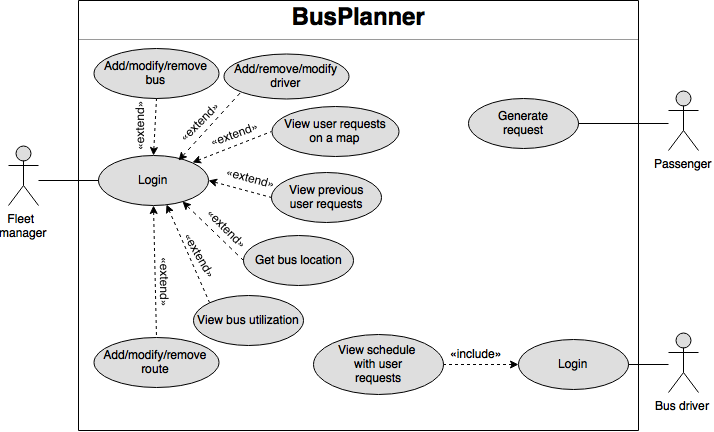
\includegraphics[width=15cm]{Use_cases}
	\caption{BusPlanner use case}
\end{figure}
\subsection{Use case description}
\subsubsection{Passenger}
\begin{table}[H]
	\centering
	\begin{tabular}{| m{3.5cm} | m{9.5cm} |}
		\hline
		\textbf{Name} & Generate request [\hyperlink{Generate_request}{Sequence diagram}]\\
		\hline
		\textbf{Actor} & Passenger\\
		\hline
		\textbf{Entry conditions} & No entry conditions.\\
		\hline
		\textbf{Flow of Events} & 
		\begin{enumerate}
			\item Open web page.
			\item Select a starting bus stop.
			\item Select an ending bus stop.
			\item Check bus availability.
		\end{enumerate}\\
		\hline
		\textbf{Exit Conditions} & Passenger gets confirmation.\\
		\hline
		\textbf{Exceptions} & No bus/seat available.\\
		\hline
	\end{tabular}
\end{table}
This use case does not correspond to any user story because our user requests will be simulated. So users will not actually be able to generate requests for a bus.

In the real world users can request a bus only if they are at a bus stop (or near one). The bus driver will be able to see the request and realize how many passengers will be at each bus stop. Requests are useful also for fleet managers, whose duty will be to assign a bus (buses are of two different sizes) to a route based on the number of requests on that same route. 

The routes are five and we cannot change them. The only thing that can change is the type of bus that is assigned to a route every day.
\newpage
\subsubsection{Fleet manager}
\begin{itemize}
	\item \hypertarget{Login_fm} Login:
\begin{table}[H]
	\centering
	\begin{tabular}{| m{3.5cm} | m{9.5cm} |}
		\hline
		\textbf{Name} & Login [\hyperlink{FmLoginSeq}{Sequence diagram}]\\
		\hline
		\textbf{Actor} & Fleet manager\\
		\hline
		\textbf{Entry conditions} & No entry condition.\\
		\hline
		\textbf{Flow of Events} & 
		\begin{enumerate}
			\item Web page opened. 
			\item Enter credentials.
			\item "Login" button pressed.
		\end{enumerate}\\
		\hline
		\textbf{Exit Conditions} & Homepage is shown.\\
		\hline
		\textbf{Exceptions} & Wrong credentials.\\
		\hline
	\end{tabular}
\end{table}
\begin{figure}[H]
	\centering
	\includegraphics[height=13cm]{FmLogin}
\end{figure}
\item \hypertarget{AddBus} Add bus:
\begin{table}[H]
	\centering
	\begin{tabular}{| m{3.5cm} | m{9.5cm} |}
		\hline
		\textbf{Name} & Add bus [\hyperlink{FmAddBusSeq}{Sequence diagram}]\\
		\hline
		\textbf{Actor} & Fleet manager\\
		\hline
		\textbf{Entry conditions} & Fleet manager is logged in.\\
		\hline
		\textbf{Flow of Events} & 
		\begin{enumerate}
			\item Open buses page. 
			\item Form is filled with bus technical details. 
			\item Submit button pressed.
		\end{enumerate}\\
		\hline
		\textbf{Exit Conditions} & Database confirmation and buses page shown.\\
		\hline
		\textbf{Exceptions} & Wrong information is entered.\\
		\hline
	\end{tabular}
\end{table}
\begin{figure}[H]
	\centering
	\includegraphics[height=13cm]{FmAddBus}
\end{figure}
\item \hypertarget{ModifyBus} Modify bus:
\begin{table}[H]
	\centering
	\begin{tabular}{| m{3.5cm} | m{9.5cm} |}
		\hline
		\textbf{Name} & Modify bus [\hyperlink{FmModifyBusSeq}{Sequence diagram}]\\
		\hline
		\textbf{Actor} & Fleet manager\\
		\hline
		\textbf{Entry conditions} & Fleet manager is logged in.\\
		\hline
		\textbf{Flow of Events} & 
		\begin{enumerate}
			\item Open buses page.
			\item Bus is selected. 
			\item Form with bus technical details is modified. 
			\item Submit button pressed.
		\end{enumerate}\\
		\hline
		\textbf{Exit Conditions} & Database confirmation and buses page shown.\\
		\hline
		\textbf{Exceptions} & Wrong information is entered.\\
		\hline
	\end{tabular}
\end{table}
\begin{figure}[H]
	\centering
	\includegraphics[height=13cm]{FmModifyBus}
\end{figure}
\newpage
\item \hypertarget{RemoveBus} Remove bus:
\begin{table}[H]
	\centering
	\begin{tabular}{| m{3.5cm} | m{9.5cm} |}
		\hline
		\textbf{Name} & Remove bus [\hyperlink{RemoveBusSeq}{Sequence diagram}]\\
		\hline
		\textbf{Actor} & Fleet manager\\
		\hline
		\textbf{Entry conditions} & Fleet manager is logged in.\\
		\hline
		\textbf{Flow of Events} & 
		\begin{enumerate}
			\item Open buses page.
			\item Bus is selected. 
			\item "Delete" button pressed.
		\end{enumerate}\\
		\hline
		\textbf{Exit Conditions} & Bus is removed and buses page is shown.\\
		\hline
		\textbf{Exceptions} & Bus not found.\\
		\hline
	\end{tabular}
\end{table}
\begin{figure}[H]
	\centering
	\includegraphics[height=13cm]{FmRemoveBus}
\end{figure}
\item \hypertarget{AddDriver} Add driver:
\begin{table}[H]
	\centering
	\begin{tabular}{| m{3.5cm} | m{9.5cm} |}
		\hline
		\textbf{Name} & Add driver [\hyperlink{AddDriverSeq}{Sequence diagram}]\\
		\hline
		\textbf{Actor} & Fleet manager\\
		\hline
		\textbf{Entry conditions} & Fleet manager is logged in.\\
		\hline
		\textbf{Flow of Events} & 
		\begin{enumerate}
			\item Open drivers page. 
			\item Form is filled with driver's technical details. 
			\item Submit button pressed.
		\end{enumerate}\\
		\hline
		\textbf{Exit Conditions} & Database confirmation and drivers page shown.\\
		\hline
		\textbf{Exceptions} & Wrong information is entered.\\
		\hline
	\end{tabular}
\end{table}
\begin{figure}[H]
	\centering
	\includegraphics[height=13cm]{FmAddDriver}
\end{figure}
\item \hypertarget{ModifyDriver} Modify driver:
\begin{table}[H]
	\centering
	\begin{tabular}{| m{3.5cm} | m{9.5cm} |}
		\hline
		\textbf{Name} & Modify driver [\hyperlink{ModifyDriverSeq}{Sequence diagram}]\\
		\hline
		\textbf{Actor} & Fleet manager\\
		\hline
		\textbf{Entry conditions} & Fleet manager is logged in.\\
		\hline
		\textbf{Flow of Events} & 
		\begin{enumerate}
			\item Open drivers page.
			\item Driver is selected. 
			\item Form with driver's technical details is modified. 
			\item Submit button pressed.
		\end{enumerate}\\
	\hline
\textbf{Exit Conditions} & Database confirmation and drivers page shown.\\
\hline
\textbf{Exceptions} & Wrong information is entered.\\
\hline
	\end{tabular}
\end{table}
\begin{figure}[H]
	\centering
	\includegraphics[height=13cm]{FmModifyDriver}
\end{figure}
\item \hypertarget{DeleteDriver} Remove driver:
\begin{table}[H]
	\centering
	\begin{tabular}{| m{3.5cm} | m{9.5cm} |}
		\hline
		\textbf{Name} & Remove driver [\hyperlink{RemoveDriverSeq}{Sequence diagram}]\\
		\hline
		\textbf{Actor} & Fleet manager\\
		\hline
		\textbf{Entry conditions} & Fleet manager is logged in.\\
		\hline
		\textbf{Flow of Events} & 
		\begin{enumerate}
			\item Open drivers page.
			\item Driver is selected. 
			\item "Delete" button pressed.
		\end{enumerate}\\
	\hline
\textbf{Exit Conditions} & Driver is removed and drivers page is shown.\\
\hline
\textbf{Exceptions} & Driver not found.\\
\hline
	\end{tabular}
\end{table}
\begin{figure}[H]
	\centering
	\includegraphics[height=13cm]{FmRemoveDriver}
\end{figure}
\item \hypertarget{Mapping_user_requests_fm} View user requests on a map:
\begin{table}[H]
	\centering
	\begin{tabular}{| m{3.5cm} | m{9.5cm} |}
		\hline
		\textbf{Name} & View user requests on a map [\hyperlink{ViewUserRequestsSeq}{Sequence diagram}]\\
		\hline
		\textbf{Actor} & Fleet manager\\
		\hline
		\textbf{Entry conditions} & Fleet manager is logged in.\\
		\hline
		\textbf{Flow of Events} & 
		\begin{enumerate}
			\item Open user requests page. 
		\end{enumerate}\\
		\hline
		\textbf{Exit Conditions} & The fleet manager is able to see the user requests on a map.\\
		\hline
		\textbf{Exceptions} & Data is not available.\\
		\hline
	\end{tabular}
\end{table}
\begin{figure}[H]
	\centering
	\includegraphics[width=14cm]{FmViewUserRequests}
\end{figure}
\newpage
\item \hypertarget{PreviousUserRequestsFm} View previous user requests:
\begin{table}[H]
	\centering
	\begin{tabular}{| m{3.5cm} | m{9.5cm} |}
		\hline
		\textbf{Name} & View previous user requests [\hyperlink{View_previous_user_requests_fm_seq}{Sequence diagram}]\\
		\hline
		\textbf{Actor} & Fleet manager\\
		\hline
		\textbf{Entry conditions} & Fleet manager is logged in.\\
		\hline
		\textbf{Flow of Events} & 
		\begin{enumerate}
			\item Open user requests page.
		\end{enumerate}\\
		\hline
		\textbf{Exit Conditions} & Fleet manager is able to see the previous users requests in a table.\\
		\hline
		\textbf{Exceptions} & Data is not available.\\
		\hline
	\end{tabular}
\end{table}
\begin{figure}[H]
	\centering
	\includegraphics[width=14cm]{FmViewPreviousUserRequests}
\end{figure}
\newpage
\item \hypertarget{Get_bus_location_fm} Get buses location:
\begin{table}[H]
	\centering
	\begin{tabular}{| m{3.5cm} | m{9.5cm} |}
		\hline
		\textbf{Name} & Get bus location [\hyperlink{GetBusLocationSeq}{Sequence diagram}]\\
		\hline
		\textbf{Actor} & Fleet manager\\
		\hline
		\textbf{Entry conditions} & Fleet manager is logged in.\\
		\hline
		\textbf{Flow of Events} & 
		\begin{enumerate}
			\item From the homepage click on \textit{Buses} button.
		\end{enumerate}\\
		\hline
		\textbf{Exit Conditions} & The fleet manager is able to view the buses location on a map.\\
		\hline
		\textbf{Exceptions} & Data not available.\\
		\hline
	\end{tabular}
\end{table}
\begin{figure}[H]
	\centering
	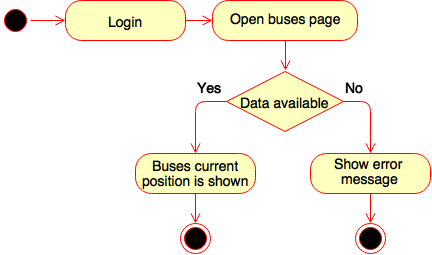
\includegraphics[width=14cm]{FmGetBusLocation}
\end{figure}
\newpage
\item \hypertarget{View_bus_utilization_fm} View routes utilization:
\begin{table}[H]
	\centering
	\begin{tabular}{| m{3.5cm} | m{9.5cm} |}
		\hline
		\textbf{Name} & View bus utilization [\hyperlink{View_bus_utilization_fm_seq}{Sequence diagram}]\\
		\hline
		\textbf{Actor} & Fleet manager\\
		\hline
		\textbf{Entry conditions} & Fleet manager is logged in.\\
		\hline
		\textbf{Flow of Events} & 
		\begin{enumerate}
			\item From the homepage click on \textit{Statistics} button.
		\end{enumerate}\\
		\hline
		\textbf{Exit Conditions} & The fleet manager is able to view the utilization of the company's routes.\\
		\hline
		\textbf{Exceptions} & Data not available.\\
		\hline
	\end{tabular}
\end{table}
\begin{figure}[H]
	\centering
	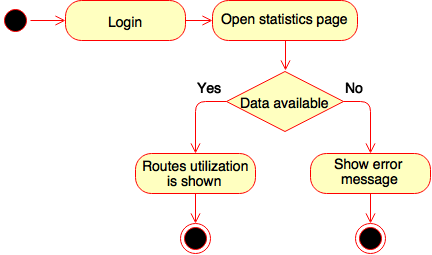
\includegraphics[width=14cm]{FmViewRoutesUtilization}
\end{figure}
\newpage
\item \hypertarget{AddRoute} Add route:
\begin{table}[H]
	\centering
	\begin{tabular}{| m{3.5cm} | m{9.5cm} |}
		\hline
		\textbf{Name} & Add route [\hyperlink{AddRouteSeq}{Sequence diagram}]\\
		\hline
		\textbf{Actor} & Fleet manager\\
		\hline
		\textbf{Entry conditions} & Fleet manager is logged in.\\
		\hline
		\textbf{Flow of Events} & 
		\begin{enumerate}
			\item Open routes page. 
			\item Form is filled with route's technical details. 
			\item Submit button pressed.
		\end{enumerate}\\
	\hline
\textbf{Exit Conditions} & Database confirmation and routes page shown.\\
\hline
\textbf{Exceptions} & Wrong information is entered.\\
\hline
	\end{tabular}
\end{table}
\begin{figure}[H]
	\centering
	\includegraphics[height=13cm]{FmAddRoute}
\end{figure}
\item \hypertarget{DeleteRoute} Remove route:
\begin{table}[H]
	\centering
	\begin{tabular}{| m{3.5cm} | m{9.5cm} |}
		\hline
		\textbf{Name} & Remove route [\hyperlink{DeleteRouteSeq}{Sequence diagram}]\\
		\hline
		\textbf{Actor} & Fleet manager\\
		\hline
		\textbf{Entry conditions} & Fleet manager is logged in.\\
		\hline
		\textbf{Flow of Events} & 
		\begin{enumerate}
			\item Open routes page.
			\item Route is selected. 
			\item "X" button pressed.
		\end{enumerate}\\
	\hline
\textbf{Exit Conditions} & Route is removed and routes page is shown.\\
\hline
\textbf{Exceptions} & Route not found.\\
\hline
	\end{tabular}
\end{table}
\begin{figure}[H]
	\centering
	\includegraphics[height=13.5cm]{FmDeleteRoute}
\end{figure}
\end{itemize}
\subsubsection{Bus driver}
\begin{itemize}
	\item \hypertarget{Login_bd} Login:
	\begin{table}[H]
		\centering
		\begin{tabular}{| m{3.5cm} | m{9.5cm} |}
			\hline
			\textbf{Name} & Login [\hyperlink{Login_bd_seq}{Sequence diagram}]\\
			\hline
			\textbf{Actor} & Bus driver\\
			\hline
			\textbf{Entry conditions} & No entry condition.\\
			\hline
			\textbf{Flow of Events} & 
			\begin{enumerate}
				\item Web page opened. 
				\item Enter credentials.
				\item "Login" button pressed.
			\end{enumerate}\\
		\hline
	\textbf{Exit Conditions} & Homepage is shown.\\
\hline
\textbf{Exceptions} & Wrong credentials.\\
\hline
		\end{tabular}
	\end{table}
\begin{figure}[H]
	\centering
	\includegraphics[height=13cm]{BdLogin}
\end{figure}
	\item \hypertarget{View_schedule_bd} View schedule:
	\begin{table}[H]
		\centering
		\begin{tabular}{| m{3.5cm} | m{9.5cm} |}
			\hline
			\textbf{Name} & View schedule with user requests [\hyperlink{View_schedule_bd_seq}{Sequence diagram}]\\
			\hline
			\textbf{Actor} & Bus driver\\
			\hline
			\textbf{Entry conditions} & Bus driver is logged in.\\
			\hline
			\textbf{Flow of Events} & 
			\begin{enumerate}
				\item Respective web page is opened. 
				\item Read data from database. 
				\item Information is shown on the screen.
			\end{enumerate}\\
			\hline
			\textbf{Exit Conditions} & Bus driver is able to view his/her schedule with all the user requests he/she needs to satisfy.\\
			\hline
			\textbf{Exceptions} & Data not available.\\
			\hline
		\end{tabular}
	\end{table}
\begin{figure}[H]
	\centering
	\includegraphics[width=14cm]{BdViewSchedule}
\end{figure}
\end{itemize}
\newpage
\subsubsection{Sequence diagrams}
\begin{itemize}
	\item \hypertarget{Generate_request} Passenger generates a request:
	\begin{figure}[H]
		\centering
		\includegraphics[width=14cm]{UserGenerateRequest}
	\end{figure}
\newpage
	\item \hypertarget{FmLoginSeq} Fleet manager login:
	\begin{figure}[H]
		\centering
		\includegraphics[width=14cm]{FmLoginSeq}
	\end{figure}
\newpage
	\item \hypertarget{FmAddBusSeq} Add bus:
	\begin{figure}[H]
		\centering
		\includegraphics[width=14cm]{FmAddBusSeq}
	\end{figure}
\newpage
\item \hypertarget{FmModifyBusSeq} Modify bus:
\begin{figure}[H]
	\centering
	\includegraphics[width=14cm]{FmModifyBusSeq}
\end{figure}
\newpage
\item \hypertarget{RemoveBusSeq} Remove bus:
\begin{figure}[H]
	\centering
	\includegraphics[width=14cm]{FmRemoveBusSeq}
\end{figure}
\newpage
\item \hypertarget{AddDriverSeq} Add driver:
\begin{figure}[H]
	\centering
	\includegraphics[width=14cm]{FmAddDriverSeq}
\end{figure}
\newpage
\item \hypertarget{ModifyDriverSeq} Modify driver:
\begin{figure}[H]
	\centering
	\includegraphics[width=14cm]{FmModifyDriverSeq}
\end{figure}
\newpage
\item \hypertarget{RemoveDriverSeq} Remove driver:
\begin{figure}[H]
	\centering
	\includegraphics[width=14cm]{FmRemoveDriverSeq}
\end{figure}
\newpage
\item \hypertarget{ViewUserRequestsSeq} View user requests on a map:
\begin{figure}[H]
	\centering
	\includegraphics[width=14cm]{FmViewUserRequestsSeq}
\end{figure}
\item \hypertarget{View_previous_user_requests_fm_seq} View previous user requests:
\begin{figure}[H]
	\centering
	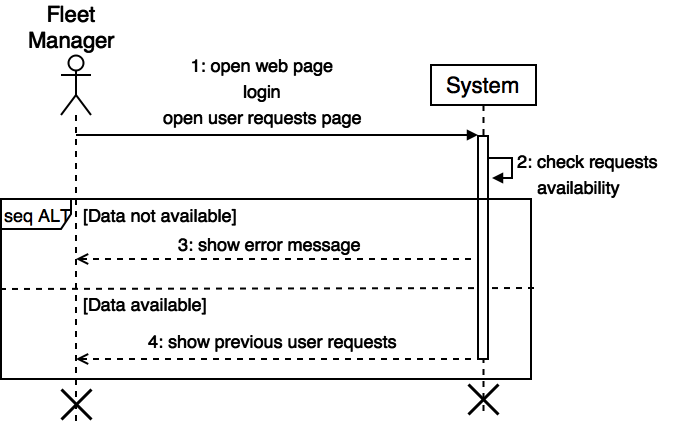
\includegraphics[width=14cm]{FmViewPreviousUserRequestsSeq}
\end{figure}
\newpage
\item \hypertarget{GetBusLocationSeq} Get buses location:
\begin{figure}[H]
	\centering
	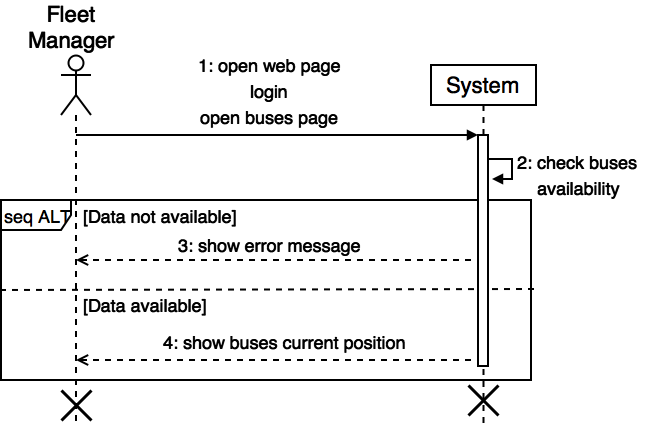
\includegraphics[width=14cm]{FmGetBusLocationSeq}
\end{figure}
\item \hypertarget{View_bus_utilization_fm_seq} View routes utilization:
\begin{figure}[H]
	\centering
	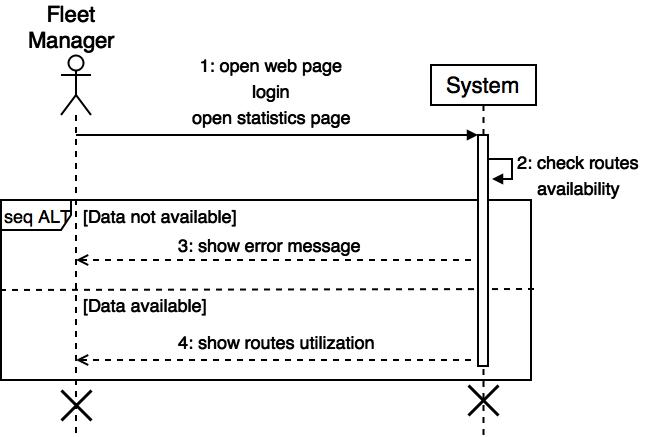
\includegraphics[width=14cm]{FmViewRoutesUtilizationSeq}
\end{figure}
\newpage
\item \hypertarget{AddRouteSeq} Add route:
\begin{figure}[H]
	\centering
	\includegraphics[width=14cm]{FmAddRouteSeq}
\end{figure}
\newpage
\item \hypertarget{DeleteRouteSeq} Delete route:
\begin{figure}[H]
	\centering
	\includegraphics[width=14cm]{FmDeleteRouteSeq}
\end{figure}
\newpage
\item \hypertarget{Login_bd_seq} Bus driver login:
\begin{figure}[H]
	\centering
	\includegraphics[width=14cm]{BdLoginSeq}
\end{figure}
\newpage
\item \hypertarget{View_schedule_bd_seq} View schedule:
\begin{figure}[H]
	\centering
	\includegraphics[width=14cm]{BdViewScheduleSeq}
\end{figure}
\end{itemize}
	\section{NONFUNCTIONAL REQUIREMENTS}
This section presents the nonfunctional requirements of our BusPlanner project, which describe the behavior of the system. We decided to divide them into 7 main categories.
\subsection{Usability}
\begin{itemize}
	\item The application must be mobile responsive.
	\item The seat reservation should be done in the minimum number of steps possible.
	\item No fancy GUI.
	\item Correct and up to date information.
	\item Presenting data in a visible and understandable way.	
\end{itemize}
\subsection{External Libraries}
\begin{itemize}
	\item Our application makes usage of external libraries such as Bootstrap.
\end{itemize}
\subsection{Compatibility issue}
\begin{itemize}
	\item The application is suggested to work only with the deployed version of the used libraries. Updated versions might bring incompatibilities. 
	\item The maps being used should offer the possibility to work with PHP and SQL.
\end{itemize}
\subsection{Security}
\begin{itemize}
	\item Only users of the application are allowed to use the project. 
	\item The application needs to protect C.I.A elements (Confidentiality, Integrity and Availability) of user and nobody can see and change information of others.
\end{itemize}
\subsection{Availability}
Considering that the application:
\begin{itemize}
	\item Can pave the way for users to take a bus as soon as possible with the aim of saving their time.
	\item Can make it easier for users to take a bus from everywhere in bus timetable.
	\item Can have friendly interface for users.
	\item Performance should provide the user a fast experience using the application.
	\item Has to handle user\textquotesingle s request all the time using any device with an Internet connection and an installed web browser.
\end{itemize}
\subsection{Uptime and data redundancy}
The BusPlanner application should guarantee high availability and data redundancy. Still, since the application will be created in the context of the DSD course, our team will not build nor require any dedicated infrastructure for it and so estimating and proving exact value for data redundancy and uptime is not possible; however, in the case there\textquotesingle s the chance to build and test a dedicated infrastructure, an uptime of at least 99.99\% is desirable along with at least one database replication.
\subsection{Performances}
The application has to be able to manage a high volume of requests. Since this application will be created in the context of the DSD course, our team will not build nor require any dedicated infrastructure for it. Furthermore, it is impossible to estimate and prove the exact value for performances. However, it should be easy to update it and improve it if needed. 
\end{document}